%%%%%%%%%%%%%%%%%%%%%%%%%%%%%%%%%%%%%%%%%%%%%%%%%%%%%%%%%%%%%%%%%%%%%%%%%%%%%%%%
%Tutorial slides on Python.
%
% Author: FOSSEE 
% Copyright (c) 2009, FOSSEE, IIT Bombay
%%%%%%%%%%%%%%%%%%%%%%%%%%%%%%%%%%%%%%%%%%%%%%%%%%%%%%%%%%%%%%%%%%%%%%%%%%%%%%%%

\documentclass[14pt,compress]{beamer}
%\documentclass[draft]{beamer}
%\documentclass[compress,handout]{beamer}
%\usepackage{pgfpages} 
%\pgfpagesuselayout{2 on 1}[a4paper,border shrink=5mm]

% Modified from: generic-ornate-15min-45min.de.tex
\mode<presentation>
{
  \usetheme{Warsaw}
  \useoutertheme{infolines}
  \setbeamercovered{transparent}
}

\usepackage[english]{babel}
\usepackage[latin1]{inputenc}
%\usepackage{times}
\usepackage[T1]{fontenc}
\usepackage{amsmath}

% Taken from Fernando's slides.
\usepackage{ae,aecompl}
\usepackage{mathpazo,courier,euler}
\usepackage[scaled=.95]{helvet}

\definecolor{darkgreen}{rgb}{0,0.5,0}

\usepackage{listings}
\lstset{language=Python,
    basicstyle=\ttfamily\bfseries,
    commentstyle=\color{red}\itshape,
  stringstyle=\color{darkgreen},
  showstringspaces=false,
  keywordstyle=\color{blue}\bfseries}

%%%%%%%%%%%%%%%%%%%%%%%%%%%%%%%%%%%%%%%%%%%%%%%%%%%%%%%%%%%%%%%%%%%%%%
% Macros
\setbeamercolor{emphbar}{bg=blue!20, fg=black}
\newcommand{\emphbar}[1]
{\begin{beamercolorbox}[rounded=true]{emphbar} 
      {#1}
 \end{beamercolorbox}
}
\newcounter{time}
\setcounter{time}{0}
\newcommand{\inctime}[1]{\addtocounter{time}{#1}{\tiny \thetime\ m}}

\newcommand{\typ}[1]{\lstinline{#1}}

\newcommand{\kwrd}[1]{ \texttt{\textbf{\color{blue}{#1}}}  }

%%% This is from Fernando's setup.
% \usepackage{color}
% \definecolor{orange}{cmyk}{0,0.4,0.8,0.2}
% % Use and configure listings package for nicely formatted code
% \usepackage{listings}
% \lstset{
%    language=Python,
%    basicstyle=\small\ttfamily,
%    commentstyle=\ttfamily\color{blue},
%    stringstyle=\ttfamily\color{orange},
%    showstringspaces=false,
%    breaklines=true,
%    postbreak = \space\dots
% }


%%%%%%%%%%%%%%%%%%%%%%%%%%%%%%%%%%%%%%%%%%%%%%%%%%%%%%%%%%%%%%%%%%%%%%
% Title page
\title[Calculus]{Python for Science and Engg: Interpolation, Differentiation and Integration}

\author[FOSSEE] {FOSSEE}

\institute[IIT Bombay] {Department of Aerospace Engineering\\IIT Bombay}
\date[] {31, October 2009\\Day 1, Session 5}
%%%%%%%%%%%%%%%%%%%%%%%%%%%%%%%%%%%%%%%%%%%%%%%%%%%%%%%%%%%%%%%%%%%%%%

%\pgfdeclareimage[height=0.75cm]{iitmlogo}{iitmlogo}
%\logo{\pgfuseimage{iitmlogo}}


%% Delete this, if you do not want the table of contents to pop up at
%% the beginning of each subsection:
\AtBeginSubsection[]
{
  \begin{frame}<beamer>
    \frametitle{Outline}
    \tableofcontents[currentsection,currentsubsection]
  \end{frame}
}

\AtBeginSection[]
{
  \begin{frame}<beamer>
   \frametitle{Outline}
   \tableofcontents[currentsection,currentsubsection]
  \end{frame}
}

% If you wish to uncover everything in a step-wise fashion, uncomment
% the following command: 
%\beamerdefaultoverlayspecification{<+->}

%\includeonlyframes{current,current1,current2,current3,current4,current5,current6}

%%%%%%%%%%%%%%%%%%%%%%%%%%%%%%%%%%%%%%%%%%%%%%%%%%%%%%%%%%%%%%%%%%%%%%
% DOCUMENT STARTS
\begin{document}

\begin{frame}
  \titlepage
\end{frame}

%% \begin{frame}
%%   \frametitle{Outline}
%%   \tableofcontents
%% %  \pausesections
%% \end{frame}

\section{\typ{loadtxt}}

\begin{frame}[fragile]
  \frametitle{Array slicing}
  \begin{lstlisting}
In []: A = array([[ 1,  1,  2, -1],
                  [ 2,  5, -1, -9],
                  [ 2,  1, -1,  3],
                  [ 1, -3,  2,  7]])

In []: A[:,0]
Out[]: array([ 1,  2,  2, 1])

In []: A[1:3,1:3]
Out[]: 
array([[ 5, -1],
       [ 1, -1]])
\end{lstlisting}
\end{frame}

\begin{frame}[fragile]
  \frametitle{\typ{loadtxt}}
  \begin{itemize}
  \item Load data from a text file.
  \item Each row must have same number of values.
  \end{itemize}
\begin{lstlisting}
In []: data = loadtxt('pendulum.txt')
In []: x = data[:, 0]
In []: y = data[:, 1]
\end{lstlisting}
\end{frame}

%% \begin{frame}[fragile]
%%   \frametitle{\typ{loadtxt}}
%% \end{frame}

\section{Interpolation}
\begin{frame}[fragile]
\frametitle{Loading data (revisited)}
\begin{itemize}
  \item Given data file \typ{points.txt}.
  \item It contains x,y position of particle.
  \item Plot the given points.
%%  \item Interpolate the missing region.
\end{itemize}
\begin{lstlisting}
In []: x, y = loadtxt('points.txt',
                       unpack = True)
In []: plot(x, y, '.')
\end{lstlisting}
\end{frame}

\begin{frame}
  \frametitle{Plot}
  \begin{center}
    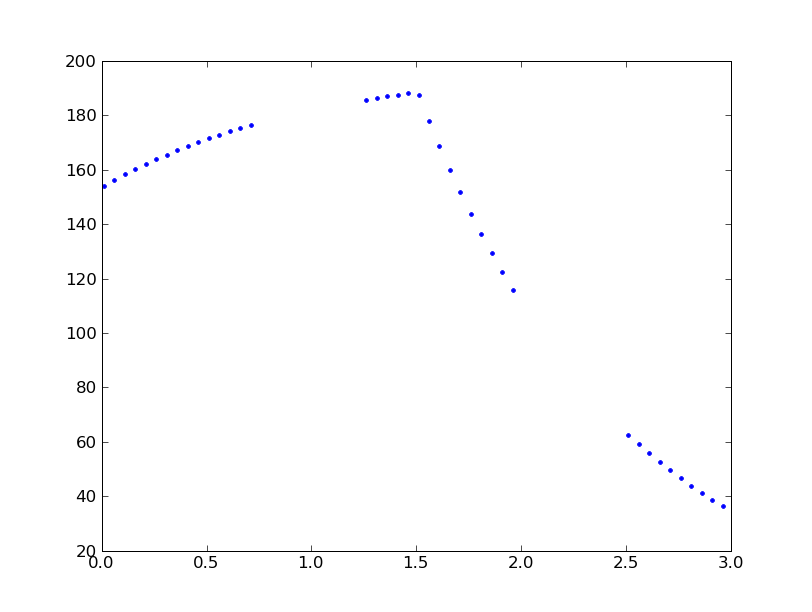
\includegraphics[height=2in, interpolate=true]{data/missing_points}
  \end{center}
\end{frame}
%% \begin{frame}[fragile]
%% \frametitle{Interpolation \ldots}
%% \begin{small}
%%   \typ{In []: from scipy.interpolate import interp1d}
%% \end{small}
%% \begin{itemize}
%% \item The \typ{interp1d} function returns a function
%% \begin{lstlisting}
%%   In []: f = interp1d(L, T)
%% \end{lstlisting}
%% \item Functions can be assigned to variables 
%% \item This function interpolates between known data values to obtain unknown
%% \end{itemize}
%% \end{frame}

%% \begin{frame}[fragile]
%% \frametitle{Interpolation \ldots}
%% \begin{lstlisting}
%% In []: Ln = arange(0.1,0.99,0.005)
%% # Interpolating! 
%% # The new values in range of old data
%% In []: plot(L, T, 'o', Ln, f(Ln), '-')
%% In []: f = interp1d(L, T, kind='cubic')
%% # When kind not specified, it's linear
%% # Others are ...
%% # 'nearest', 'zero', 
%% # 'slinear', 'quadratic'
%% \end{lstlisting}
%% \end{frame}

\begin{frame}[fragile]
\frametitle{Spline Interpolation}
\begin{small}
\begin{lstlisting}
In []: from scipy.interpolate import splrep
In []: from scipy.interpolate import splev
\end{lstlisting}
\end{small}
\begin{itemize}
\item Involves two steps
  \begin{enumerate}
  \item Find out the spline curve, coefficients
  \item Evaluate the spline at new points
  \end{enumerate}
\end{itemize}
\end{frame}

\begin{frame}[fragile]
\frametitle{\typ{splrep}}
To find the spline curve
\begin{lstlisting}
In []: tck = splrep(x, y)
\end{lstlisting}
\typ{tck} contains parameters required for representing the spline curve!
\end{frame}

\begin{frame}[fragile]
\frametitle{\typ{splev}}
To Evaluate a spline and it's derivatives
\begin{lstlisting}
In []: Xnew = arange(0.01,3,0.02)
In []: Ynew = splev(Xnew, tck)

In []: y.shape
Out[]: (40,)

In []: Ynew.shape
Out[]: (150,)
 
In []: plot(Xnew, Ynew)
\end{lstlisting}

\end{frame}

%% \begin{frame}[fragile]
%% \frametitle{Interpolation \ldots}
%% \begin{itemize}
%% \item 
%% \end{itemize}
%% \end{frame}

\begin{frame}
  \frametitle{Plot}
  \begin{center}
    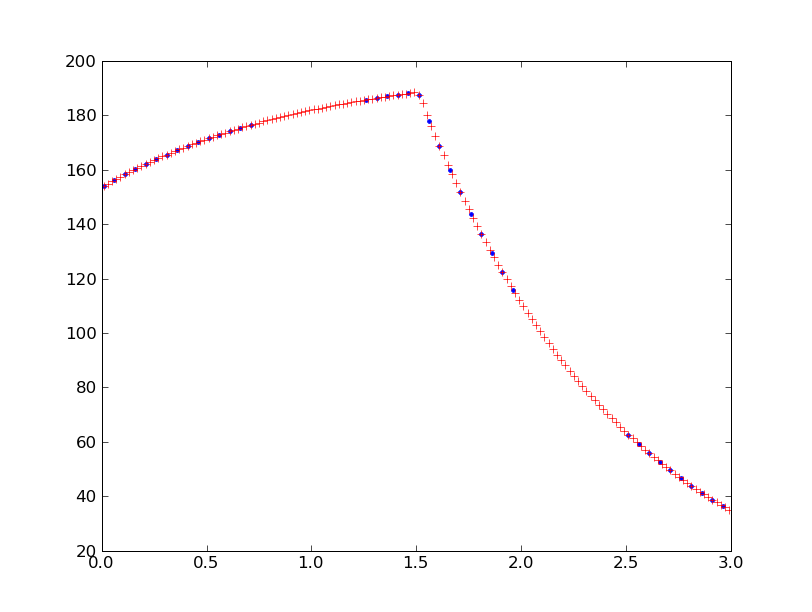
\includegraphics[height=2in, interpolate=true]{data/interpolate}
  \end{center}
\end{frame}

\section{Differentiation}

\begin{frame}[fragile]
\frametitle{Numerical Differentiation}
\begin{itemize}
\item Given function $f(x)$ or data points $y=f(x)$
\item We wish to calculate $f^{'}(x)$ at points $x$
\item Taylor series - finite difference approximations
\end{itemize}
\begin{center}
\begin{tabular}{l l}
$f(x+h)=f(x)+hf^{'}(x)$ &Forward \\
$f(x-h)=f(x)-hf^{'}(x)$ &Backward
\end{tabular}
\end{center}
\end{frame}

\begin{frame}[fragile]
\frametitle{Forward Difference}
\begin{lstlisting}
In []: x = linspace(0, 2*pi, 100)
In []: y = sin(x)
In []: deltax = x[1] - x[0]
\end{lstlisting}
Obtain the finite forward difference of y
\end{frame}

\begin{frame}[fragile]
\frametitle{Forward Difference \ldots}
\begin{lstlisting}
In []: fD = (y[1:] - y[:-1]) / deltax
In []: print len(fD)
Out[]: 99
In []: plot(x, y) 
In []: plot(x[:-1], fD)
\end{lstlisting}
\vspace{-.2in}
\begin{center}
  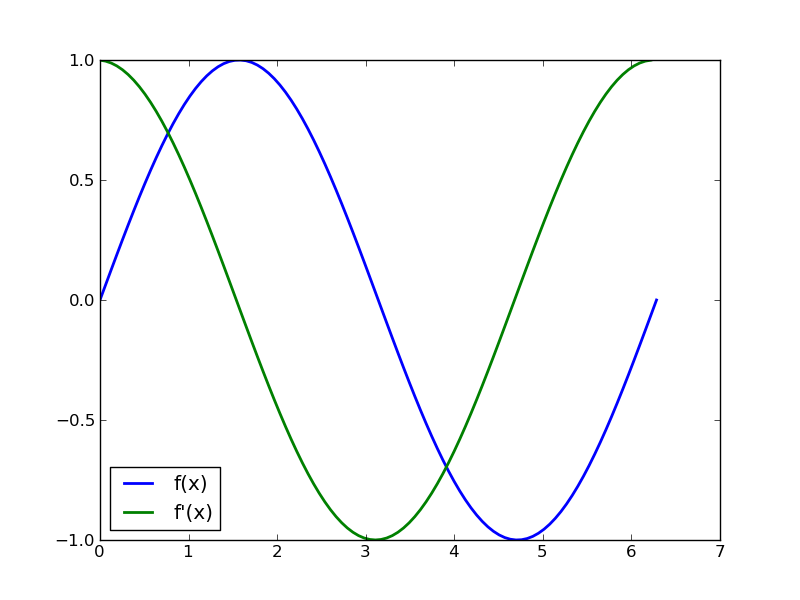
\includegraphics[height=1.8in, interpolate=true]{data/fwdDiff}
\end{center}
\end{frame}

\begin{frame}[fragile]
\frametitle{Example}
\begin{itemize}
\item Given x, y positions of a particle in \typ{pos.txt}
\item Find velocity \& acceleration in x, y directions
\end{itemize}
\small{
\begin{center}
\begin{tabular}{| c | c | c |}
\hline
$X$ & $Y$ \\ \hline
0.     &  0.\\ \hline
0.25   &  0.47775\\ \hline
0.5    &  0.931\\ \hline
0.75   &  1.35975\\ \hline
1.     &  1.764\\ \hline
1.25   &  2.14375\\ \hline
\vdots & \vdots\\ \hline
\end{tabular}
\end{center}}
\end{frame}

\begin{frame}[fragile]
\frametitle{Example \ldots}
\begin{itemize}
\item Read the file
\item Obtain an array of X, Y
\item Obtain velocity and acceleration
\item use \typ{deltaT = 0.05}
\end{itemize}
\begin{lstlisting}
In []: data = loadtxt('pos.txt')
In []: X,Y = data[:,0], data[:,1]
In []: S = array([X, Y])
\end{lstlisting}
\end{frame}


\begin{frame}[fragile]
\frametitle{Example \ldots}
\begin{lstlisting}
In []: deltaT = 0.05

In []: v = (S[:,1:]-S[:,:-1])/deltaT

In []: a = (v[:,1:]-v[:,:-1])/deltaT
\end{lstlisting}
\end{frame}

\begin{frame}[fragile]
\frametitle{Example \ldots}
Plotting Y, $v_y$, $a_y$
\begin{lstlisting}
In []: plot(Y)
In []: plot(v[1,:])
In []: plot(a[1,:])
\end{lstlisting}
\begin{center}
  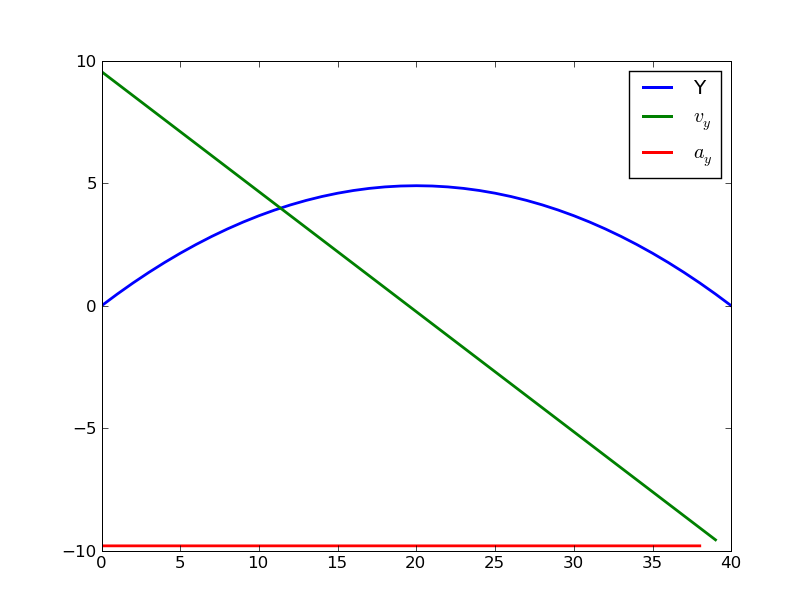
\includegraphics[height=1.8in, interpolate=true]{data/pos_vel_accel}  
\end{center}
\end{frame}

\section{Quadrature}

\begin{frame}[fragile]
\frametitle{Quadrature}

\emphbar{$\int_0^1(sin(x) + x^2)$}

\typ{In []: from scipy.integrate import quad}

\begin{itemize}
\item Inputs - function to integrate, limits
\end{itemize}
\begin{lstlisting}
In []: quad(sin(x)+x**2, 0, 1)
NameError: name 'x' is not defined
In []: x = 0
In []: quad(sin(x)+x**2, 0, 1)
\end{lstlisting}
\begin{small}
\alert{\typ{error:}}
\typ{First argument must be a callable function.}
\end{small}
\end{frame}

\begin{frame}[fragile]
\frametitle{Functions - Definition}
We have been using them all along. Now let's see how to define them.
\begin{lstlisting}
In []: def f(x):
           return sin(x)+x**2
In []: quad(f, 0, 1)
\end{lstlisting}
\begin{itemize}
\item \typ{def}
\item name
\item arguments
\item \typ{return}
\end{itemize}
\end{frame}

\begin{frame}[fragile]
\frametitle{Functions - Calling them}
\begin{lstlisting}
In [15]: f()
---------------------------------------
\end{lstlisting}
\alert{\typ{TypeError:}}\typ{f() takes exactly 1 argument}
\typ{(0 given)}
\begin{lstlisting}
In []: f(0)
Out[]: 0.0
In []: f(1)
Out[]: 1.8414709848078965
\end{lstlisting}
More on Functions later \ldots
\end{frame}

\begin{frame}[fragile]
\frametitle{Quadrature \ldots}
\begin{lstlisting}
In []: quad(f, 0, 1)
\end{lstlisting}
Returns the integral and an estimate of the absolute error in the result.
\begin{itemize}
\item \typ{dblquad}, \typ{tplquad} are available
\end{itemize}
\end{frame}

\begin{frame}
  \frametitle{Things we have learned}
  \begin{itemize}
  \item Interpolation
  \item Differentiation
  \item Functions
    \begin{itemize}
    \item Definition
    \item Calling
    \item Default Arguments
    \item Keyword Arguments
    \end{itemize}
  \item Quadrature
  \end{itemize}
\end{frame}

\end{document}

